\section{Concerns of Validity}
\label{sec:Validity}


\subsection{Alternative explanations for the downturn in tickets}

To examine the possibility that these results are driven by a secular trend, 
we repeat the regression specified in 
Section \ref{sec:Empirical_all} 
by splitting the pre-period in half. 
Because of the very heterogeneous effects by gender, 
we perform two sets of placebo checks using the regression specification from 
Section \ref{sec:Empirical_all}, 
one for males and one for females. 
The results of this analysis are displayed in 
Table \ref{tab:seas_Logit_vs_LPMx100K_placebo_regs}. 

% Logistic Regression and Linear Probability Models: Seasonal Logit and LPM x 100K Placebo Specification 

\begin{table}% [ht] 
\centering 
\begin{tabular}{l r r r r l r r l} 

\hline 
 
 & \multicolumn{5}{c}{Logistic Regression}  & \multicolumn{3}{c}{Linear Probability Model} \\ 

 \cmidrule(lr){2-6}\cmidrule(lr){7-9} 
 & \multicolumn{2}{c}{Marginal Effects} & Estimate & Standard & Sig. & Estimate & Standard & Sig. \\ 

 \cmidrule(lr){2-3} 
 &   AME &  MER  &          &  Error   &      &          &  Error   &     \\ 

\hline 
 
\multicolumn{8}{l}{\textbf{Male Drivers} (2,618,869,394 observations)} \\ 

\hline
\multicolumn{8}{l}{Model without age-policy interaction: } \\ 
Policy                   &  -0.1306        &  -0.5478       &  -0.0024        &  0.0017       &            &  -0.2109        &  0.0905       &            \\ 
\hline
\multicolumn{8}{l}{Model with age-policy interaction: } \\ 
Policy                   &  -1.0812        &  -4.1848       &  -0.0572        &  0.0540       &            &  -1.8092        &  1.0215       &            \\ 
Age 16-19 * policy   &  -1.1446        &  -2.6473       &  -0.0106        &  0.0545       &            &  -2.9360        &  1.3097       &            \\ 
Age 20-24 * policy   &  2.0266        &  4.5628       &  0.0204        &  0.0542       &            &  -0.1000        &  1.1226       &            \\ 
Age 25-34 * policy   &  3.2514        &  8.7684       &  0.0457        &  0.0542       &            &  1.3441        &  1.0507       &            \\ 
Age 35-44 * policy   &  2.8733        &  8.4706       &  0.0496        &  0.0542       &            &  1.2368        &  1.0420       &            \\ 
Age 45-54 * policy   &  3.4577        &  10.9720       &  0.0698        &  0.0542       &            &  1.9795        &  1.0375       &            \\ 
Age 55-64 * policy   &  3.5248        &  12.0052       &  0.0879        &  0.0543       &            &  2.3344        &  1.0386       &            \\ 
Age 65+ * policy   &  3.3942        &  12.9623       &  0.1316        &  0.0545       &            &  2.7337        &  1.0342       &            \\ 

\hline 

\multicolumn{8}{l}{\textbf{Female Drivers} (2,109,880,942  observations)} \\ 

\hline
\multicolumn{8}{l}{Model without age-policy interaction: } \\ 
Policy                   &  -0.1543        &  -0.8795       &  -0.0059        &  0.0027       &            &  -0.1803        &  0.0706       &            \\ 
\hline
\multicolumn{8}{l}{Model with age-policy interaction: } \\ 
Policy                   &  0.8415        &  4.3695       &  0.1696        &  0.1874       &            &  0.6983        &  0.9249       &            \\ 
Age 16-19 * policy   &  -6.8789        &  -26.4519       &  -0.1940        &  0.1879       &            &  -1.1349        &  1.0789       &            \\ 
Age 20-24 * policy   &  -6.4219        &  -23.3417       &  -0.1686        &  0.1875       &            &  -0.0914        &  0.9821       &            \\ 
Age 25-34 * policy   &  -5.7121        &  -22.0027       &  -0.1848        &  0.1875       &            &  -1.0372        &  0.9438       &            \\ 
Age 35-44 * policy   &  -5.4912        &  -21.6223       &  -0.1970        &  0.1875       &            &  -1.4878        &  0.9396       &            \\ 
Age 45-54 * policy   &  -3.7063        &  -15.7414       &  -0.1681        &  0.1875       &            &  -0.8437        &  0.9355       &            \\ 
Age 55-64 * policy   &  -2.4244        &  -11.0054       &  -0.1496        &  0.1876       &            &  -0.6454        &  0.9358       &            \\ 
Age 65+ * policy   &  -1.0624        &  -5.1866       &  -0.1028        &  0.1878       &            &  -0.3173        &  0.9345       &            \\ 

\hline 

\end{tabular} 
\caption{Placebo regressions for all offences} 
For each regression, the dependent variable is an indicator that a driver has committed  
any offence on a particular day.  
All regressions contain age category and demerit point category controls, 
as well as monthly and weekday indicator variables. 
The baseline age category comprises drivers under the age of 16. 
The heading ``Sig.'' is an abbreviation for statistical significance, with 
the symbol * denoting statistical significance at the 0.1\% level 
and ** the 0.001\% level. 
In the linear probability model, coefficients and heteroskedasticity-robust standard errors are  
multiplied by 100,000.  
\label{tab:seas_Logit_vs_LPMx100K_placebo_regs} 
\end{table} 
 


The regression results show no statistical evidence of pre-trends, 
and none of the coefficients of interest are precisely estimated. 
Moreover, the magnitude of the coefficients in both placebo regressions 
for the model without age-policy interactions are very similar 
and are far smaller than their counterparts in the real regressions; 
we argue that this is evidence of precisely estimated zeros 
given their magnitude and small standard errors.%
\footnote{% 
Even with the very large sample employed in this analysis, 
unless the effect is exactly zero in the population, 
a non-zero standard error and coefficient estimate will be still be produced. 
For a discussion on precise zeros, see 
\citet{penney2013}. 
}
%
If there were a secular trend in the pre-period driving the results of the main regressions, 
the male coefficient would have a substantially larger magnitude than the female coefficient, 
but this is not the case. 
In the set of regressions containing the age category dummies interacted with the policy variable, 
none of the interactions are statistically significant, and there is no pattern among the coefficients either.
This result contrasts with the coefficients on the age interactions for males 
in the main regression in which we observe a clear pattern: 
the effect is similar from ages 16 to 25, and then slowly declines with age. 
Overall, we do not find any convincing evidence that the effects found in the 
real main regression are an artifact of something other than the excessive speeding laws.


An alternative explanation is the idea that police leniency may have changed as a result of the law; 
we examine this possibility here. 
The introduction of additional penalties for excessive speeding may 
motivate police officers to note tickets as lesser speeding violations. 
For example, excessive speeding in zones with a limit of 60km/h 
could be marked down to a 3-point ticket, 
while excessive speeding in zones with higher limits could be reduced to a 5-point ticket. 
Three arguments speak against this possibility. 
First, police officers could behave in this fashion to avoid appearing in court 
in case the driver contests the charges.  
In Quebec, however, police officers are not required to appear in traffic court.%
\footnote{% 
See the following website (in French) for details: \texttt{https://educaloi.qc.ca/capsules/la-contestation-dune-contravention/} (Accessed July 18, 2020).}  
%
Second, a police officer aiming to be lenient would reduce the speed on a ticket 
to a level where the excessive speeding provisions would not take effect. 
% 
However, according to 
Table \ref{tab:seas_Logit_vs_LPMx100K_regs_by_points}, 
the incidence of tickets for men decreases for every category above 1 point, 
while for women it decreases for every category above 2 points. 
In other words, the categories to which the tickets would be marked down (3-point or 5-point tickets) still saw decreases.%
\footnote{% 
Note that there are no speeding violations worth 4 points under the Quebec highway safety code, and that 4-point tickets are much less common than 3-point or 5-point tickets; see 
Table \ref{tab:point_freq}.
}
% 
Finally, the overall number of tickets per driver-day still decreased (the extensive margin), 
and leniency against the provisions of the excessive speeding law 
would only affect the intensive margin of demerit points. 
We conclude it is very unlikely that a change in police leniency could be driving the results.


% Logistic Regression and Linear Probability Models: Seasonal Logit and LPM x 100K Specification by Event Month 

\begin{table}% [ht] 
\centering 
\begin{tabular}{l r r r r l r r l} 

\hline 
 
 & \multicolumn{5}{c}{Logistic Regression}  & \multicolumn{3}{c}{Linear Probability Model} \\ 

 \cmidrule(lr){2-6}\cmidrule(lr){7-9} 
 & \multicolumn{2}{c}{Marginal Effects} & Estimate & Standard & Sig. & Estimate & Standard & Sig. \\ 
 &   AME & MER &          &  Error   &      &          &  Error   &     \\ 

\hline 
 
\multicolumn{7}{l}{\textbf{Male Drivers} (5,335,033,221 observations)} \\ 

Policy Indicator          &  -4.0366        &  -16.4792       &  -0.0762        &  0.0015       &   **       &  -4.1859        &  0.0763       &   **       \\ 
Month 1                         &  9.9449        &  38.5317       &  0.1483        &  0.0047       &   **       &  8.6823        &  0.2761       &   **       \\ 
Month 2                         &  7.2862        &  27.2675       &  0.1110        &  0.0046       &   **       &  6.6386        &  0.2726       &   **       \\ 
Month 3                         &  2.2160        &  8.3591       &  0.0380        &  0.0048       &   **       &  2.2264        &  0.2683       &   **       \\ 
Month 4                         &  -4.7201        &  -17.3888       &  -0.0965        &  0.0049       &   **       &  -5.0416        &  0.2534       &   **       \\ 
Month 5                         &  -4.1329        &  -17.4499       &  -0.0969        &  0.0052       &   **       &  -4.5641        &  0.2379       &   **       \\ 
Month 6                         &  -6.4410        &  -20.9716       &  -0.1206        &  0.0047       &   **       &  -6.9509        &  0.2708       &   **       \\ 
Month 7                         &  -4.2653        &  -14.4849       &  -0.0782        &  0.0046       &   **       &  -4.4353        &  0.2648       &   **       \\ 
Month 8                         &  -6.3291        &  -22.5706       &  -0.1320        &  0.0049       &   **       &  -7.3088        &  0.2584       &   **       \\ 
Month 9                         &  -4.9332        &  -35.9259       &  -0.2503        &  0.0071       &   **       &  -6.6876        &  0.1737       &   **       \\ 
Month 10                        &  -10.5940        &  -44.5275       &  -0.3699        &  0.0057       &   **       &  -15.3145        &  0.2167       &   **       \\ 
Month 11                        &  -6.2712        &  -23.1921       &  -0.1366        &  0.0051       &   **       &  -7.2667        &  0.2609       &   **       \\ 
Month 12                        &  -2.8571        &  -10.5662       &  -0.0551        &  0.0047       &   **       &  -3.1070        &  0.2560       &   **       \\ 

\hline 

\multicolumn{7}{l}{\textbf{Female Drivers} (4,340,212,273 observations)} \\ 

Policy Indicator          &  0.8179        &  4.6888       &  0.0310        &  0.0022       &   **       &  0.8391        &  0.0611       &   **       \\ 
Month 1                         &  3.7539        &  19.1217       &  0.1063        &  0.0070       &   **       &  3.5263        &  0.2238       &   **       \\ 
Month 2                         &  2.1374        &  10.6644       &  0.0632        &  0.0069       &   **       &  2.2000        &  0.2191       &   **       \\ 
Month 3                         &  -0.4495        &  -2.3531       &  -0.0157        &  0.0074       &            &  -0.3857        &  0.2112       &            \\ 
Month 4                         &  -3.4773        &  -18.6622       &  -0.1527        &  0.0078       &   **       &  -4.0417        &  0.1945       &   **       \\ 
Month 5                         &  -3.2337        &  -19.8371       &  -0.1654        &  0.0083       &   **       &  -3.9171        &  0.1824       &   **       \\ 
Month 6                         &  -4.5281        &  -19.8371       &  -0.1654        &  0.0071       &   **       &  -4.8207        &  0.2167       &   **       \\ 
Month 7                         &  -3.8277        &  -17.3447       &  -0.1390        &  0.0071       &   **       &  -3.9811        &  0.2116       &   **       \\ 
Month 8                         &  -4.5030        &  -21.4857       &  -0.1842        &  0.0074       &   **       &  -5.3036        &  0.2072       &   **       \\ 
Month 9                         &  -2.9968        &  -32.3390       &  -0.3584        &  0.0117       &   **       &  -5.3165        &  0.1302       &   **       \\ 
Month 10                        &  -6.0362        &  -37.1693       &  -0.5268        &  0.0095       &   **       &  -10.3117        &  0.1611       &   **       \\ 
Month 11                        &  -4.3594        &  -22.6167       &  -0.1978        &  0.0080       &   **       &  -5.2484        &  0.2036       &   **       \\ 
Month 12                        &  -2.1026        &  -10.5533       &  -0.0772        &  0.0072       &   **       &  -2.1935        &  0.2059       &   **       \\ 

\hline 

\end{tabular} 
\caption{Regressions with indicators for month since policy change} 
For each regression, the dependent variable is an indicator that a driver has committed  
any offence on a particular day.  
All regressions contain age category and demerit point category controls, 
as well as monthly and weekday indicator variables. 
The baseline age category comprises drivers under the age of 16. 
The heading ``Sig.'' is an abbreviation for statistical significance, with 
the symbol * denoting statistical significance at the 0.1\% level 
and ** the 0.001\% level. 
In the linear probability model, coefficients and heteroskedasticity-robust standard errors are  
multiplied by 100,000.  
\label{tab:seas_Logit_vs_LPMx100K_event_month_regs} 
\end{table} 
 



An increase in police vigilance during the implementation of the policy 
could also have affected the magnitude of the results. 
Indeed, it would have increased the number of tickets written in that period, 
which would result in an underestimation of the effect. 
% 
We investigated this possibility by including separate dummy variables
for the first 12 months after the change in laws. 
These results are shown in 
Table \ref{tab:seas_Logit_vs_LPMx100K_event_month_regs}. 
The variable called ``Policy Indicator'' equals 1 for the entire period after
the law came into effect. 
In each of the subsequent 12 months, the effect of the policy is measured 
as the sum of the ``Policy Indicator'' coefficient 
and the coefficient for the numbered month. 
% 
These monthly policy effects are plotted over the two-year period 
after the policy change in Figure \ref{fig:event_study}.
% 
For male drivers, the probability of obtaining any ticket increased by 
$0.00450$ and $0.00245$ percentage points in the first two months of the policy
but decreased by the third month. 
The program had maximum effectiveness over the last half of 2008, 
with a decrease of $0.00729$ percentage points in the twelfth month,
not far from the overall policy effect of $0.00597$ in 
Table \ref{tab:seas_Logit_vs_LPMx100K_regs}. 
% 
For female drivers, the pattern was similar, except that the magnitude 
of the decline was smaller and the effect in the second year was a
small increase in magnitude. 
% 
Together, this suggests some combination of an increase in police vigilance 
and a learning curve over the course of a year. 

\begin{figure}
\centering
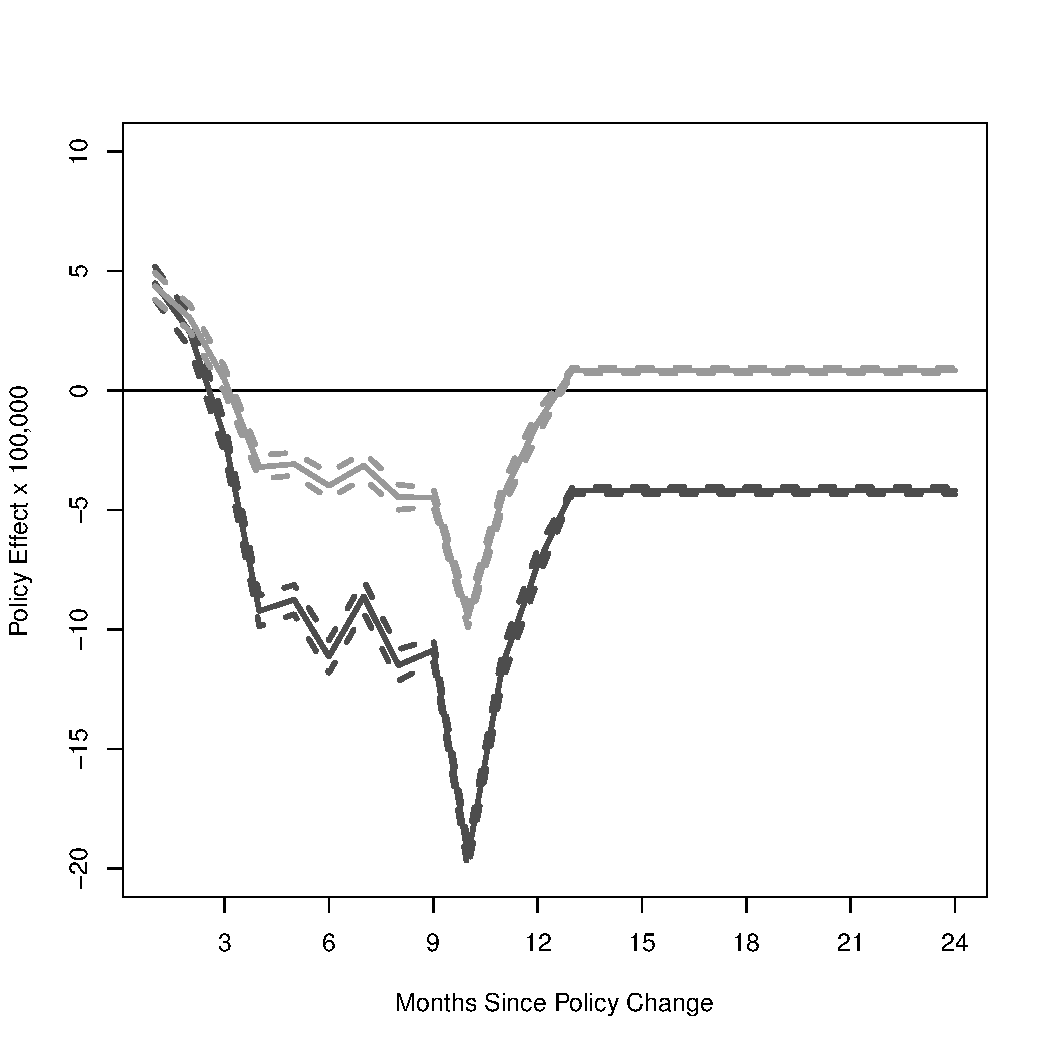
\includegraphics[width=0.8\textwidth]{Figures/Event_Study}
\caption{Monthly pattern of the policy effects \\
The points along the path reflect the net effect measured by 
the coefficients for the ``Policy Indicator'' 
and the corresponding ``Month'' indicator, 
shown in Table \ref{tab:seas_Logit_vs_LPMx100K_event_month_regs}, 
multiplied by 100,000. 
The black lines represent the effects for males 
and the grey lines those for females. 
The dashed lines are 95\% confidence bands. 
}\label{fig:event_study}
\end{figure}



During about the last third of the sample period after the policy change, 
the province of Quebec introduced a photo radar pilot. 
It started issuing tickets for speeding on August 19, 2009. 
We do not believe this had a substantial effect on driver behaviour for several reasons. 
First, the number of photo radar machines was very small: 
there were 15 in the entire province of Quebec, 
which had a population of approximately 8 million people at the time.%
\footnote{% 
Of these 15, 6 were for speeding, 6 were for red light violations, and 3 were mobile 
\citep{bisson2020}.
}  
%
Second, during the pilot, 
the photo radar machines were placed in plain sight, 
and warning signs were placed ahead of them to clearly alert drivers of their location.

One last consideration is that, in April 2008, 
the Quebec government also introduced new legislation 
banning the use of handheld mobile devices while driving. 
This new violation associated with 3 demerit points could have 
increased the number of violations in the dataset. 
In 2008, there were 18,254 violations for this charge and 48,835 in 2009 
% 
\citep[table 1.3]{SAAQ2010}.
%  
Despite the introduction of these new violations, 
we still observe a decrease in the total number of violations, 
suggesting our results could be underestimating the real impact of the excessive speeding laws.



\subsection{Statistical properties}

For our empirical analysis, we estimated regressions using
both the linear probability model
and logistic regression; both models have limitations
which we address here. 

Concerns may be raised about the mathematical properties of estimates 
derived from the use of linear probability models. 
For example, 
\citet{horraceoaxaca2006}
claim that predicted probabilities outside of the $[0,1]$ interval 
indicate bias and inconsistency of the linear probability model regression estimates. 
For all regressions conducted in our paper, 
no predicted probabilities fall outside of this interval, 
assuaging this concern. 
Furthermore, the absence of negative predictions is not a product of chance: 
because the explanatory variables in our regressions are all categorical variables, 
the predictions are essentially proportions, 
rather than linear predictions from continuous variables. 
This helps to mitigate the usual criticism of the linear probability model. 

We also estimated a model with driver-specific fixed effects
to account for the possibility that the tendency to get tickets
is not independent between drivers within the same category. 
To facilitate the calculation, we aggregated the data across the time dimension
rather than across drivers
to achieve the same degree of data compression as in the regressions reported above.
We augmented these estimates with cluster-robust standard error estimates 
by clustering on the individual drivers. 
For our purposes, this model has severe limitations. 
First, the fixed effects annihilate the age and gender categories, 
which we found were strongly related to driving behaviour
and worth analyzing in a model. 
Second, and more importantly, 
the remaining variation in our dataset comprises 
only the demerit-point balance indicators and the policy indicator. 
Although still of interest, including demerit-point balances is problematic because 
this variable is a moving average of a variable closely related to the dependent variable:
the number of demerit points for a ticket instead of the indicator for a ticket. 
Still, we found a negative policy effect that was decreasing 
in the current demerit-point balance;
however, the estimates were orders of magnitude larger 
than those recorded in the models without fixed effects. 
This finding is explained by the bias introduced by the direct relationship between the demerit-point balance and the dependent variable, 
which we confirmed with simulation evidence. 


Another issue is the relative rarity of the events 
(the driver-days where the dependent variable is equal to 1 rather than 0). 
\citet{kingzheng2001}
show that rare events cause estimated probabilities to be biased downwards for logit estimation 
(in the case where ones are rare relative to zeros). 
The level of the rare events bias is a function of 
the frequency of events relative to the total sample size: 
for example, a sample size of 1,000 with 2 events (0.2\% of the sample) 
may suffer from rare events bias, 
but a sample size of 100,000 with 200 events (also 0.2\%) may not. 
To examine whether rare events bias potentially exists in our analysis, 
we conduct a Monte Carlo experiment as follows. 
We set up a simulation using an effect size that is similar to the regression involving females but uses a much smaller sample size: 
if rare events bias appears absent, 
it should not be a concern of note in the real regression 
which has a sample 100 times larger. 
The simulation has 1,000 repetitions. 
For each, we generate a dataset with 43,390,582 observations 
where 0.00369\% of observations in the pre-period have an event, 
and 0.004449\% in the post-period. 
The effect size of interest is the difference between these two numbers, which is 0.000759\%. 
The results are as follows. 
We find no statistical evidence of rare events bias: 
the mean effect size of the simulations is also 0.000759\% 
and the estimates are tightly distributed, 
with the 25th percentile being equal to 0.000620\%, 
and the 75th percentile to 0.000889\%. 
Moreover, the statistical power is healthy, 
with 30.1\% of the samples producing statistically significant results 
for the effect size at the 0.001\% level; 
this is despite the simulation using a sample size only one one-hundredth 
that of the sample used in the analysis. 
We conclude that it is unlikely that rare events bias 
is influencing the results in a statistically meaningful fashion.



